\chapter{Related Work}


\section{Benchmarks of NoSQL Databases}

A wealth of literature is available related to the performance comparison of different NoSQL databases over RDF data. Instead of introducing a part of these papers, we focus on the foundations of the measurements, the benchmark frameworks. In the following, each section represents a benchmark particularly connecting to RDF data models. Finally, Section \ref{sec:benchmark_conclusions} compares the frameworks, and by drawing conclusions based on the benchmarks, it also contains the main concepts on which we will rely in our search.

\subsection{Yahoo!~Cloud Serving Benchmark}

The \textit{Yahoo!~Cloud Serving Benchmark} was elaborated in order to compare performance of the new generation
of cloud data serving systems~\cite{ycsb}. The framework proposes different workloads by assigning
different distributions to them that determine the operation to perform --- get or put --- and the record from the data model to be read or written. In other words, the particular distributions specify the exact numbers of read or update queries in a workload, and also affect the choosing of records on which the workload operates. In order to demonstrate, Figure 1 %todo insert pic from 5
represents the available distributions and number of choices per records.

\subsection{Berlin SPARQL Benchmark}

The Berlin SPARQL Benchmark (from now on BSBM) is settled in an e-commerce use case in which a set of products
is offered by different vendors and consumers have posted reviews about these products on various review sites~\cite{berlin}. Taken scalability into consideration, BSBM proposes an arbitrary increased model size. Similarly to YCSB, BSBM concentrates on read and update operations as well, as it defines three different use cases and a suite of benchmark queries in each of them~\cite{berlin_specification}. The queries were elaborated to simulate realistic, real-life workloads.

In contrast to YCSM, BSBM defines particular performance metrics that relate mainly to the query execution times from different perspectives. For example, the most important metrics are the following:
\begin{itemize}
	\item{Queries per Second}: It equals to the number of queries that executed properly by the system within a second.
	\item{Query Mixes per Hour}: Denotes the number of \textit{mixed} queries with different parameters that evaluated within an hour.
	\item{Overall Runtime}: The overall time that a certain amount of query mixes required.
\end{itemize}


\subsection{DBpedia SPARQL Benchmark}
DBpedia SPARQL Benchmark proposes datasets in various sizes derived from the DBpedia~\cite{dbpedia_data} knowledge base, and perform measurements on real queries that were issued against existing RDF data~\cite{dbpedia}. Similarly to BSBM, DBpedia also defines metrics to provide a more precise performance analysis. These are the same as in the case of BSBM: \textit{Query Mixes per Hour}, and \textit{Queries per Second}. Furthermore, DBpedia investigates the characterization of the models as well and calculates the average in- and outdegree, the number of nodes and distinct IRIs, however, it uses these measurements to judge and maintain the generated model to be similar to the original data set. As a consequence, DBpedia does not explore model and performance correlations neither.

\subsection{SP$^2$Bench}
The SPARQL Performance Benchmark (SP$^2$Bench) is designed to test the most common SPARQL constructs,
operator constellations, and a broad range of RDF data access patterns~\cite{sp2bench}. Instead of defining a sequence of use case motivated queries, the framework proposes various queries that cover specific RDF data management approaches.

SP$^2$Bench is based on the \textit{Digital Bibliography and Library Project} (commonly known as \textit{dblp}) which provides an open bibliographic information on major computer science publications~\cite{dblp}. The benchmark queries are not explicitly evaluated over the \textit{dblp} dataset, since SP$^2$Bench uses arbitrarily large, artificially generated models for the measurements, however, these models are constructed to follow real-life characteristics that were found in the original \textit{dblp} dataset, such as a power-law distribution.

Similarly to BSBM, SP$^2$Bench also measures additional performance related metrics besides execution time, such as disk storage cost, memory consumption, data loading time, success rates, and every one them captures different aspects of evaluations.


\subsection{Train Benchmark Framework}

\begin{figure}[!ht]
	\centering
	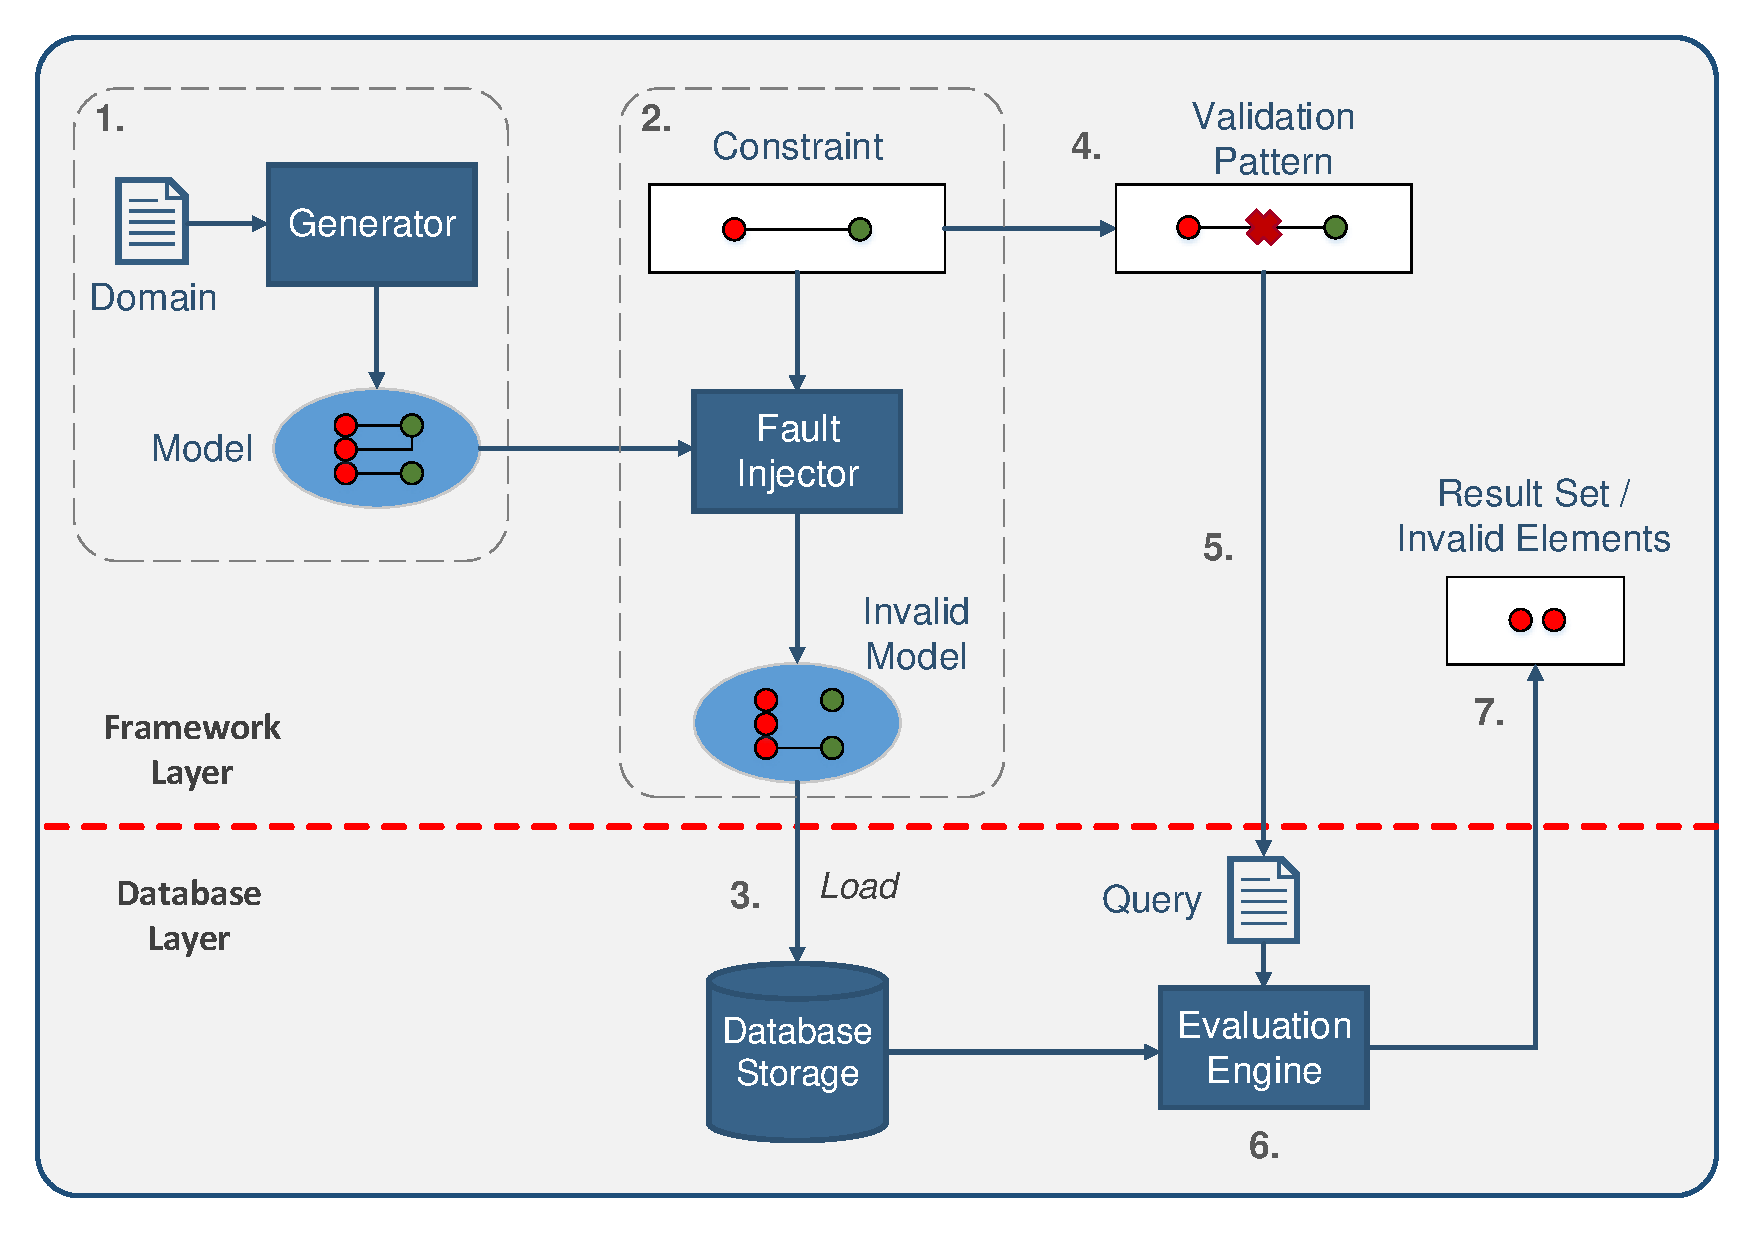
\includegraphics[width=150mm, keepaspectratio]{figures/functionality.pdf}
	\caption{An overview of Train Benchmark.}
	\label{fig:functionality}
\end{figure}

Short overview: well-formedness constraints + model validations, transformations.\\
Extended scope: RDF, EMF, SQL, Graphml.
Domain disadvantages. Emphasize this as common problems.

What is not mentioned: workflow, components, tools, detailed generator


The original domain of the Train Benchmark framework (introduced in \ref{section:metamodel} is not applicable for our goals to analyze graph queries, and study model - performance relationships. The main problems connecting to the domain are summarized in the following list:
\begin{enumerate}
	\item The original domain is not related to a real-life model, which leads to the fact that the cardinalities of the elements and their relationships do not follow a real model's characteristic, therefore, the measurement results of different tools cannot be claimed to be representative in a real-life use case. \label{item:railway_problem1}
	\item Besides the origin of the domain, the second problem is that the artificially generated models do not cover a well-known topology or degree distribution that can be observed in actual networks. \label{item:railway_problem2}
	\item Finally, the generated models of Train Benchmark are not capable to attach arbitrary connections between the elements. \label{item:railway_problem3}
\end{enumerate}

Obviously, problem \ref{item:railway_problem2} is relevant to the generator component's insufficiency, since a representative distribution can be achieved independently on the domain, however, in order to generate arbitrary distributions, it is essential to guarantee a solution for problem \ref{item:railway_problem3}.

Problem \ref{item:railway_problem3} requires some explanation. In order to construct graphs with different degree distributions, it is an essential expectation of the domain to contain self-references, thus indicating that any of the vertices can be adjacent. In addition, the presence of a self-reference should be also interpretable conceptually in the domain. 

Considering the original domain, the type \textsf{Segment} represents the majority of the elements, however---without breaking the original meaning of the domain---we cannot make connection between any of the segments.


To summarize, a new domain is necessary that is related to a real-life model, and also suited to use for generating different distributions.


\subsection{Conclusions} \label{sec:benchmark_conclusions}

One common attribute of the previously introduced benchmark frameworks is that they lack precise analysis of searching connection between model characteristic and evaluation performance. In these frameworks, it is not supported to assess a tool's performance on different topologies, still using the same domain. Generally, the frameworks propose the generation of variously large models, thus investigating scalability, however, they do not focus on modifying the internal structures of the models, and generate different topologies, even in the same size.

%todo more? metrics? prob dist? use case?
